	La distribucion uniforme es una de las mas conocidas, y como la nomal, una de las mas presentes en la realidad.
	Esta distribuci\'on es muy simple. B\'asicamente plantea que tenemos un espacio muestral $S=\{m_1, m_2, ... ,m_n\}$, $(\forall m_i \in S$,  $P(m_i)=1/n)$, osea, todos los sucesos tiene la misma probabilidad de ocurrir. 
			
	El ejemplo mas cl\'asico para entender esta distribuci\'on, es el lanzamiento de un dado de 6 caras (no cargado), en donde $S = \{1, 2, 3, 4, 5, 6\}$ y cada elemento tiene la misma probabilidad de salir, osea $ \frac{1}{6} $.
			
\subsubsection*{Tiempo de espera de un colectivo}

	Otro ejemplo un poco m\'as interesante, es si tomamos un rango de tiempo, y medimos el tiempo de espera de un colectivo en ese rango. Si bien este ejemplo depender\'a mucho sobre que l\'inea de colectivo se haga el muestreo, se puede tomar un rango en particular en el cual sabemos que el tiempo de espera no ser\'a mayor o menor a eso. A continuaci\'on, se presenta un histograma sobre un \textit{dataset} sobre los tiempos de cierto colectivo en el rango de 5 minutos a 30 minutos.
		
	\begin{figure}[H]
	  \begin{center}
	    %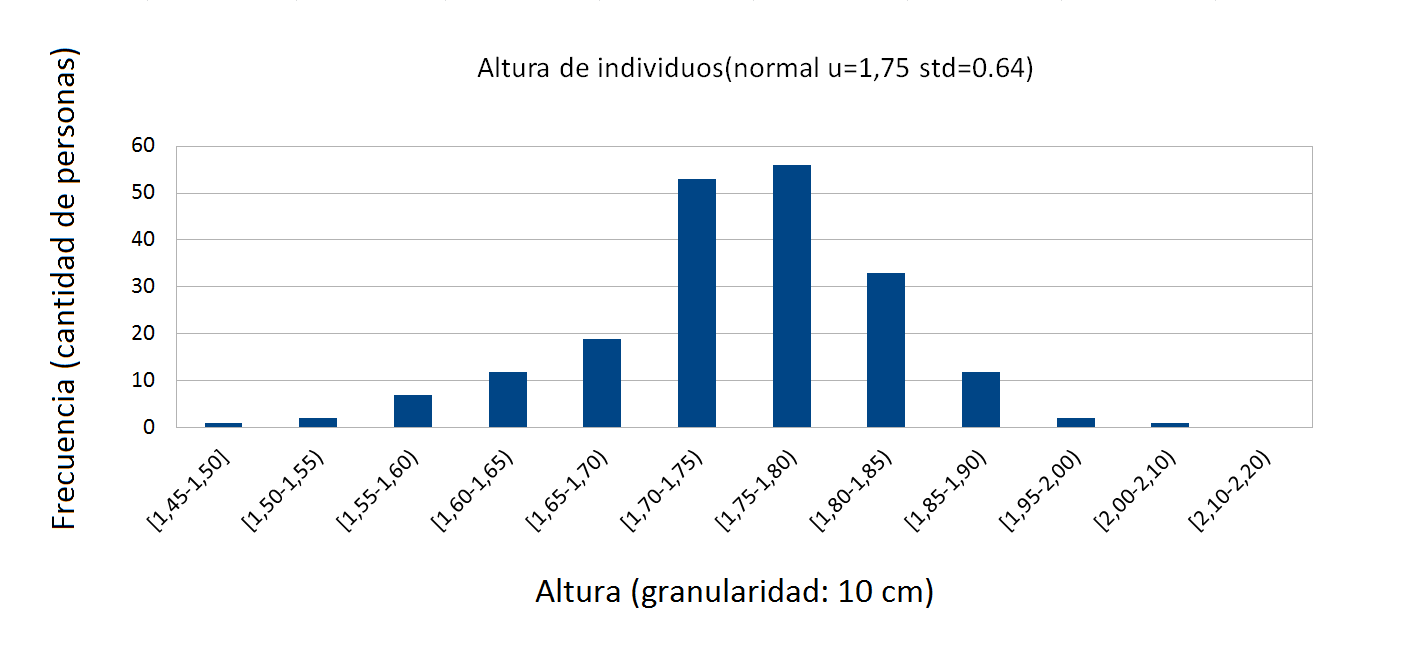
\includegraphics[scale=.41,angle=-90]{imgenes/normal_ejemplo1.png}
	    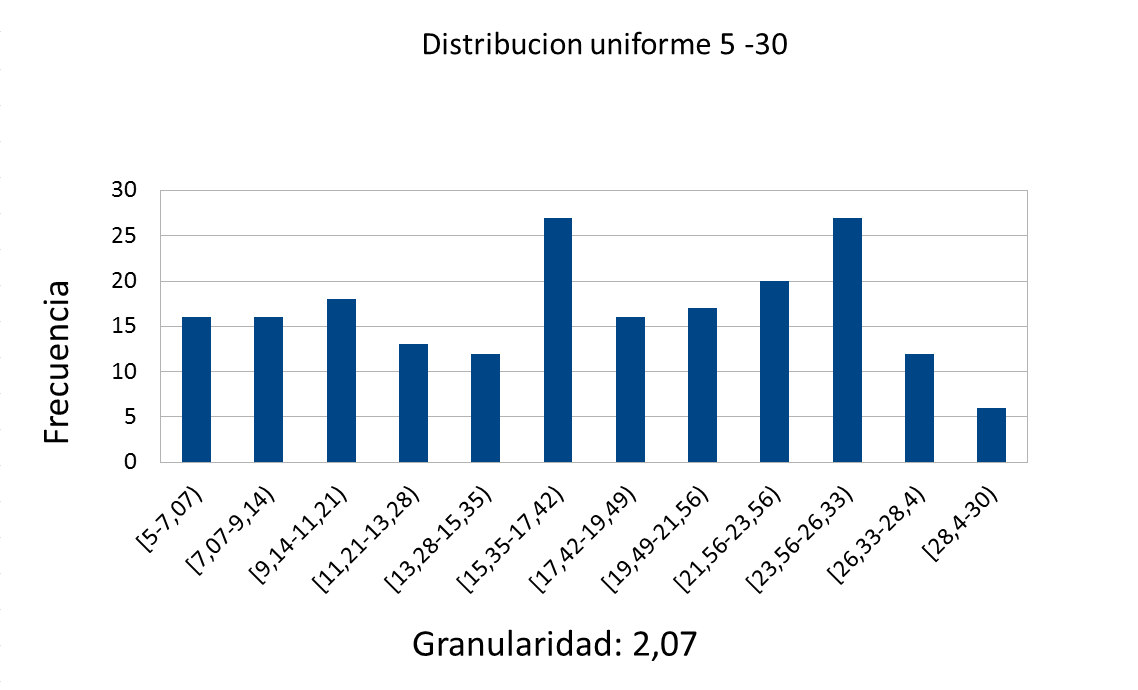
\includegraphics[scale=.40]{imagenes/uniforme_ejemplo.png}
	    \caption{Histograma tiempos de espera de colectivo} 
	    \label{fig:normal_ejemplo1}
	  \end{center}
	\end{figure}